\documentclass{jarticle}
\usepackage[dvipdfmx]{graphicx}

\title{ソフトウェア設計及び実験\\課題タイトル}
\author{出席番号 氏名}
\date{日付}

\begin{document}
\maketitle

\section{実習の目的}
%
実習の目的は以下のとおり.\\
なお, {\LaTeX}の詳細については, 参考文献~\cite{okumura},~\cite{matsuda}などを参照すること. 

\section{原理・アルゴリズム}
%
\subsection{文字のスタイルについて}
%
Abc. \texttt{Abc}. \textbf{Abc}. 

\subsection{段落について}

段落と段落の間は一行以上の空行を入れると, 段落が変わる. 

段落1段落1段落1段落1段落1段落1段落1段落1段落1段落1段落1段落1段落1
段落1段落1段落1段落1段落1段落1段落1段落1段落1段落1段落1段落1段落1

段落2段落2段落2段落2段落2段落2段落2段落2段落2段落2段落2段落2段落2
段落2段落2段落2段落2段落2段落2段落2段落2段落2段落2段落2段落2段落2

段落の行頭は一文字分下がる. 下げたくないときには$\backslash$noindent命令を
用いるとよい. 

\noindent
段落3段落3段落3段落3段落3段落3段落3段落3段落3段落3段落3段落3段落3
段落3段落3段落3段落3段落3段落3段落3段落3段落3段落3段落3段落3段落3

\subsection{箇条書きについて}
%
\subsubsection{Itemize環境}

\begin{itemize}
\item アイテム1

アイテム1アイテム1アイテム1アイテム1アイテム1アイテム1

\item アイテム2

アイテム2アイテム2アイテム2アイテム2アイテム2アイテム2

\item アイテム3

アイテム3アイテム3アイテム3アイテム3アイテム3アイテム3
\end{itemize}

\subsubsection{Description環境}
%
\begin{description}

\item[Item1 : ] アイテム1アイテム1アイテム1アイテム1アイテム1アイテム1

\item[Item2 : ] アイテム2アイテム2アイテム2アイテム2アイテム2アイテム2

\item[Item3 : ] アイテム3アイテム3アイテム3アイテム3アイテム3アイテム3

\end{description}

\subsection{数式について}
%
本文中に数式を埋め込むには, $f(t) = \sum_{i=1}^{n} x_{i} \exp \lambda_{i} t$
とすればよい. 
また, 独立した式として扱いたい場合は, 

\begin{equation}
f(t) = \sum_{i=1}^{n} x_{i} \exp \lambda_{i} t
\end{equation}
%
とする. 数式モード中で使えるコマンドの詳細は教科書や{\LaTeX}の本を参照すること. 

\subsection{図(EPSファイル)の張り込みについて}
%
\begin{figure}
\begin{center}
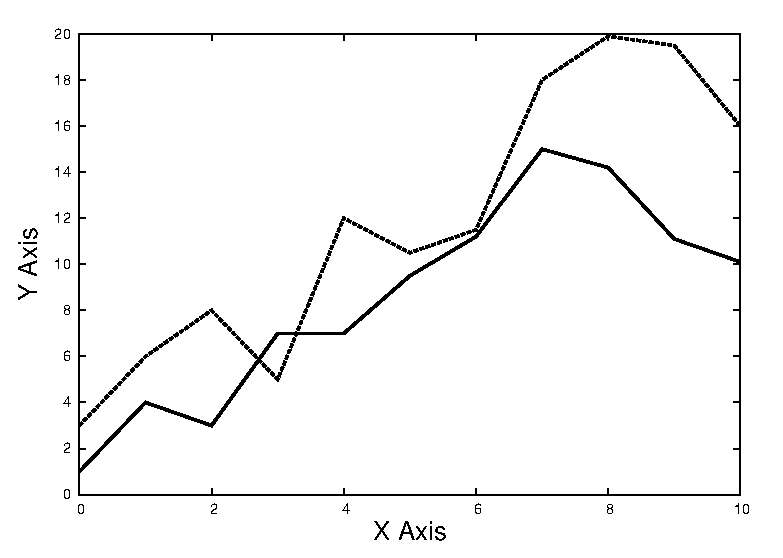
\includegraphics[scale=0.30]{graph.eps}
\caption{GNUPLOTによるグラフの張り込み例}
\label{fig:graph}
\end{center}
\end{figure}

図~\ref{fig:graph}は, グラフ作成ツールGNUPLOTを用いてデータをグラフ化し, 
svg形式で保存したものを, 図形処理ツールDiaを用いて加工したもの. 
最終的には, ファイル名'graph.eps'として, EPS形式で保存している

\subsection{表について}
%
表~\ref{table:table1}は, あるデータを表にしたものである. 

\begin{table}
\caption{表の例}
\label{table:table1}
\begin{center}
\begin{tabular}{|c|c|c|}\hline
$x$ & $y_{1}$ & $y_{2}$ \\ \hline
0.0 & 1.0 & 3.0 \\ \hline
1.0 & 5.0 & 5.0 \\ \hline
2.0 & 4.0 & 9.0 \\ \hline
3.0 & 10.0 & 15.0 \\\hline
\end{tabular}
\end{center}
\end{table}

\section{実験および結果}
%
\subsection{実験の目的}
%
\subsection{実験計画}
%
\subsection{結果}
%
\section{考察}
%
\section{課題}
%
\subsection{課題1}
%
\subsection{課題2}
%
\section{おわりに} 
%
\begin{thebibliography}{99}
%
\bibitem{okumura} 奥村 晴彦: LaTeX2ε美文書作成入門 改訂第4版,  技術評論社 (2006).
%
\bibitem{matsuda} 松田七美男 : Linux活用術, 東京電機大学出版局 (1998).
%
\end{thebibliography}

\end{document}

